% --------------------------------------------------------------
% This is all preamble stuff that you don't have to worry about.
% Head down to where it says "Start here"
% --------------------------------------------------------------

\documentclass[12pt]{article}

\usepackage[margin=1in]{geometry}
\usepackage{amsmath,amsthm,amssymb}
\usepackage{graphicx} %This allows to include eps figures
\usepackage{subcaption}
\usepackage[section]{placeins}
\usepackage{layout}
\usepackage{etoolbox}
\usepackage{mathabx}
\usepackage{animate}
\usepackage{array}
% This is to include code
\usepackage{listings}
\usepackage{xcolor}
\definecolor{dkgreen}{rgb}{0,0.6,0}
\definecolor{gray}{rgb}{0.5,0.5,0.5}
\definecolor{mauve}{rgb}{0.58,0,0.82}
\lstdefinestyle{Python}{
    language        = Python,
    basicstyle      = \ttfamily,
    keywordstyle    = \color{blue},
    keywordstyle    = [2] \color{teal}, % just to check that it works
    stringstyle     = \color{green},
    commentstyle    = \color{red}\ttfamily
}

\newenvironment{conditions}
  {\par\vspace{\abovedisplayskip}\noindent\begin{tabular}{>{$}l<{$} @{${}={}$} l}}
  {\end{tabular}\par\vspace{\belowdisplayskip}}

\newcommand{\N}{\mathbb{N}}
\newcommand{\Z}{\mathbb{Z}}

\newenvironment{theorem}[2][Theorem]{\begin{trivlist}
\item[\hskip \labelsep {\bfseries #1}\hskip \labelsep {\bfseries #2.}]}{\end{trivlist}}
\newenvironment{lemma}[2][Lemma]{\begin{trivlist}
\item[\hskip \labelsep {\bfseries #1}\hskip \labelsep {\bfseries #2.}]}{\end{trivlist}}
\newenvironment{exercise}[2][Exercise]{\begin{trivlist}
\item[\hskip \labelsep {\bfseries #1}\hskip \labelsep {\bfseries #2.}]}{\end{trivlist}}
\newenvironment{reflection}[2][Reflection]{\begin{trivlist}
\item[\hskip \labelsep {\bfseries #1}\hskip \labelsep {\bfseries #2.}]}{\end{trivlist}}
\newenvironment{proposition}[2][Proposition]{\begin{trivlist}
\item[\hskip \labelsep {\bfseries #1}\hskip \labelsep {\bfseries #2.}]}{\end{trivlist}}
\newenvironment{corollary}[2][Corollary]{\begin{trivlist}
\item[\hskip \labelsep {\bfseries #1}\hskip \labelsep {\bfseries #2.}]}{\end{trivlist}}



\begin{document}

% --------------------------------------------------------------
%                         Start here
% --------------------------------------------------------------

%\renewcommand{\qedsymbol}{\filledbox}

\title{Assignment 3}%replace X with the appropriate number
\author{Nalet Meinen and Pascal Wyss\\ %replace with your name
Finite Element Analysis I
}
\maketitle
\section*{Abstract}
In this assignment we examine the behaviour of a beam after being subjected to an impulse.
The goal is to extract the resonance frequency of the beam with the given dimensions and material coefficients.


% \begin{figure}[!htb]
%   \centering
%   \animategraphics[autoplay,loop,width=0.8\linewidth,trim={1mm 1mm 1mm 1mm}]{4}{pics/out/ani-}{1}{62}
%   \caption{Animation of frequency on beam}
% \end{figure}

\tableofcontents
\pagebreak
\section{Introduction}
The goal of this assignment is the analyzation of a beam attached to a wall 
and how it is related to its resonance frequencies. We want to show the analytical 
solution and after the model implemented in Abaqus. An example of this calculation 
can be used in dental implants, as the beginns to oscillate under given circumstances.

% I'm refering to something\footnote{footnotes working fine \cite{einstein}} .

\section{Methods}

\subsection{Analytical solution}
Consider a beam with the following dimensions attached to a wall in our case 
on the left end:
\begin{equation}\label{eq:1}
  L=150mm, h=2.5mm, b=20mm, E=10GPa, v=0.3, \rho=7.0E3kg.m^{-3}
\end{equation}
The resonance frequencies (inducing a bending in the direction of the dimension h) of
such a model are given by the formula:
\begin{equation}\label{eq:2}
  \frac{1}{2\pi\sqrt{12}}\alpha_i^2\sqrt{\frac{E}{\rho}}\frac{h}{L^2}
\end{equation}
Where:
\begin{conditions}
  \alpha_0 & $1.875,\alpha_1=4.695,\alpha_2=7.85,...,\alpha_i=(2i+1)\frac{\pi}{2} \enspace  for \, i>2$ \\
  E     &  Young's modulus \\
  \rho  &  density of the material \\   
  h     &  height of the cross-section of the beam \\
  L     &  length of the beam
\end{conditions}
\noindent Using our values for $\alpha_0$:
\begin{equation}\label{eq:3}
  f_0 = \frac{1}{2\pi\sqrt{12}}1.875^2\sqrt{\frac{10 \cdot 10^3 Pa}{7\cdot10^3 
  \frac{kg}{m^3}}}\frac{2.5 \cdot 10^3 m}{(150 \cdot 10^3 m)^2} = 21.451 \, Hz
\end{equation}
\newpage
\subsection{Frequency mode on Beam}

\begin{figure}[!htb]
  \centering
  \begin{subfigure}{.5\textwidth}
    \centering
    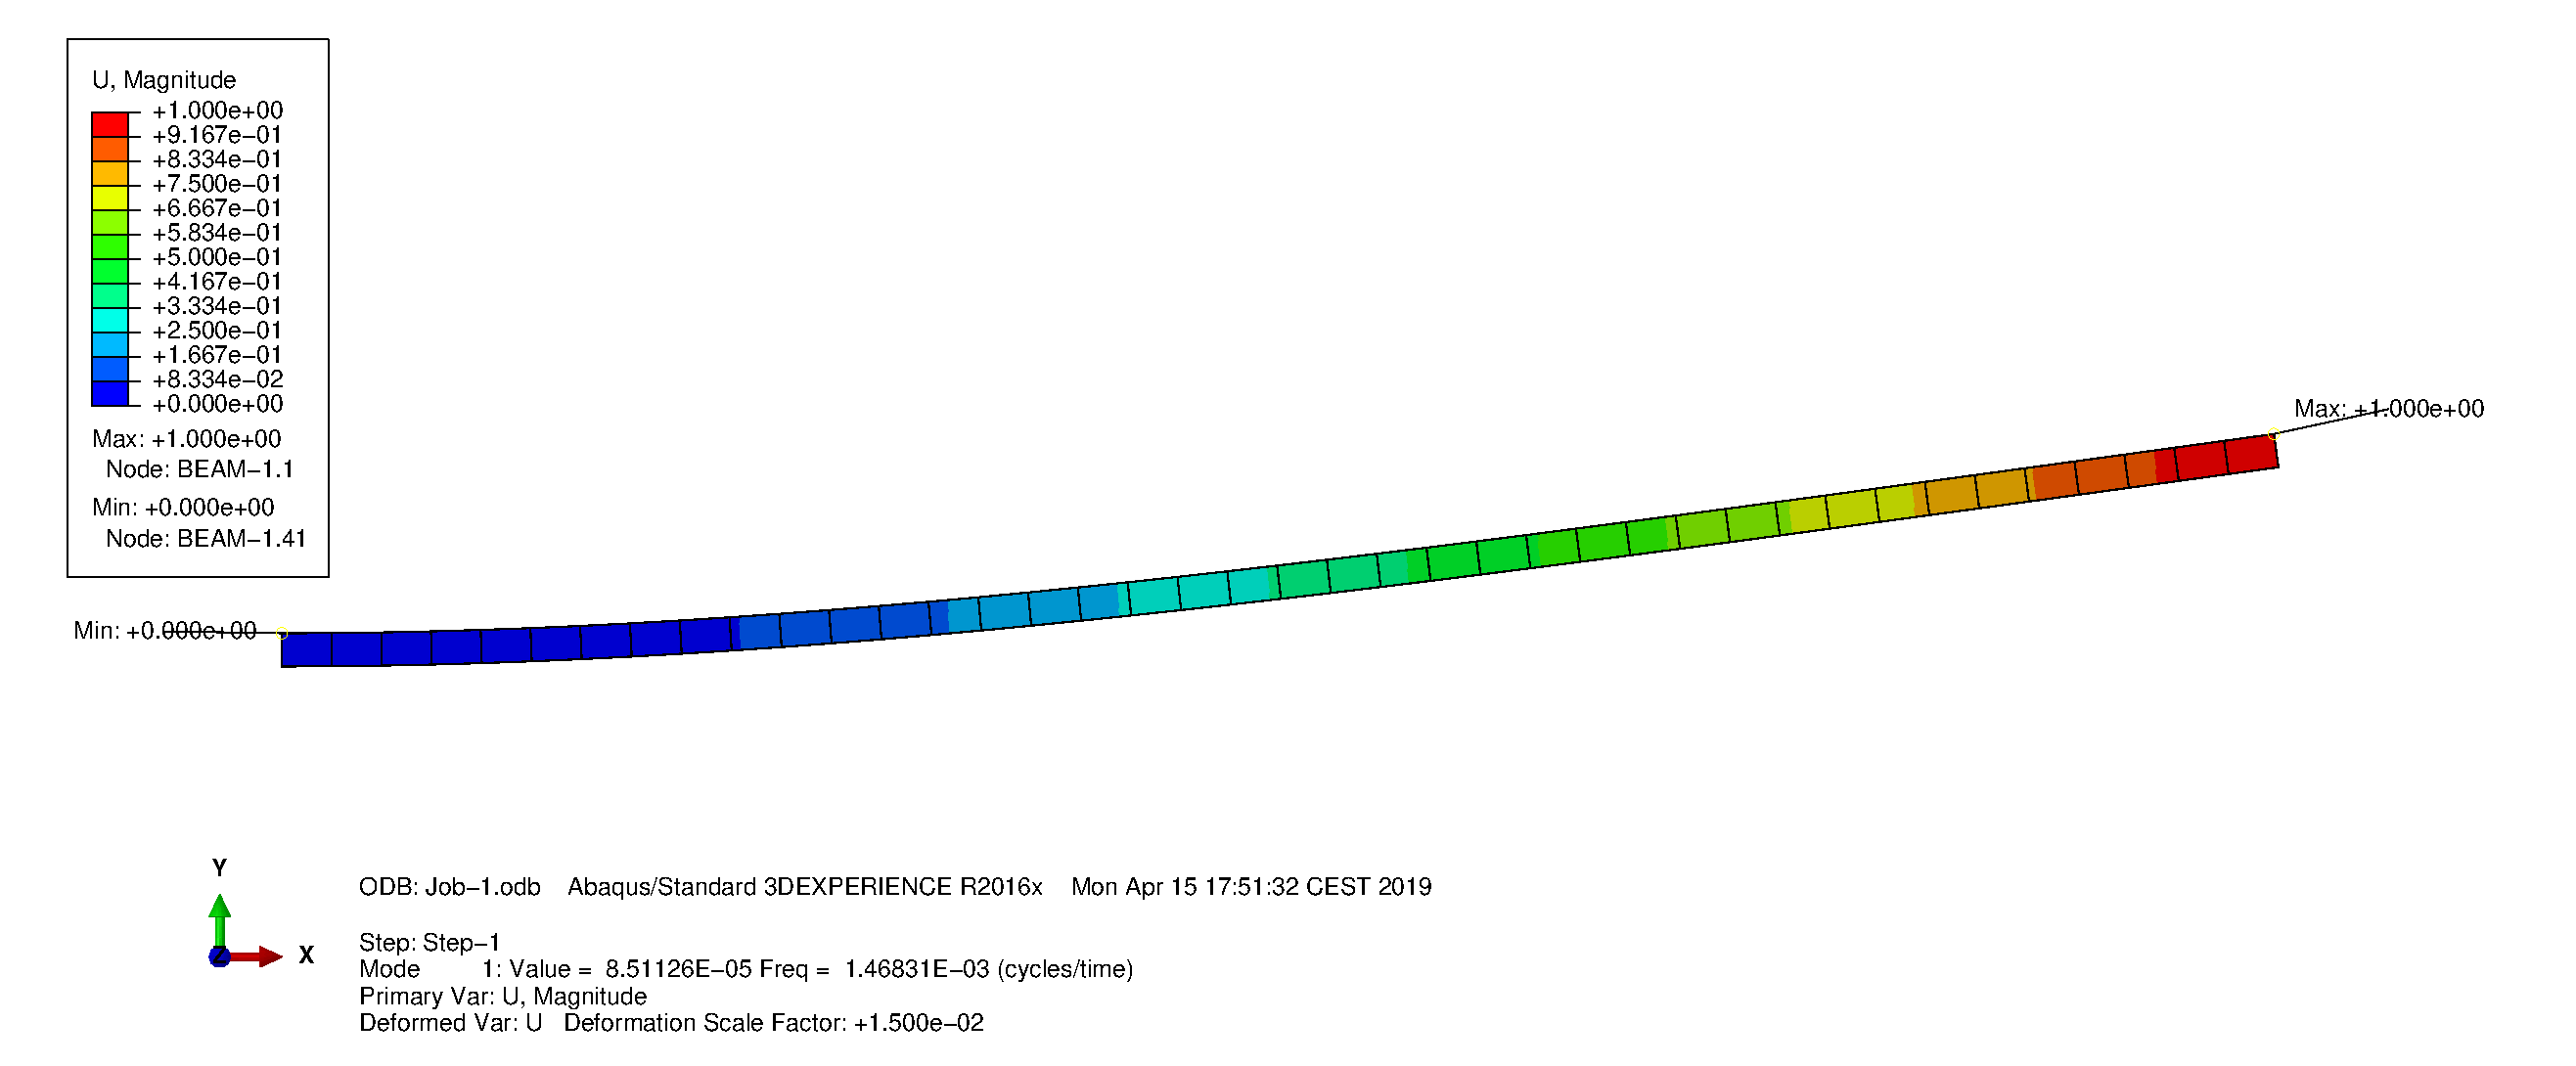
\includegraphics[width=0.95\linewidth]{pics/Beam_1_CPS4R}
    \caption{calculated frequency with CPS4R: 14.6 Hz}
  \end{subfigure}%
  \begin{subfigure}{.5\textwidth}
    \centering
    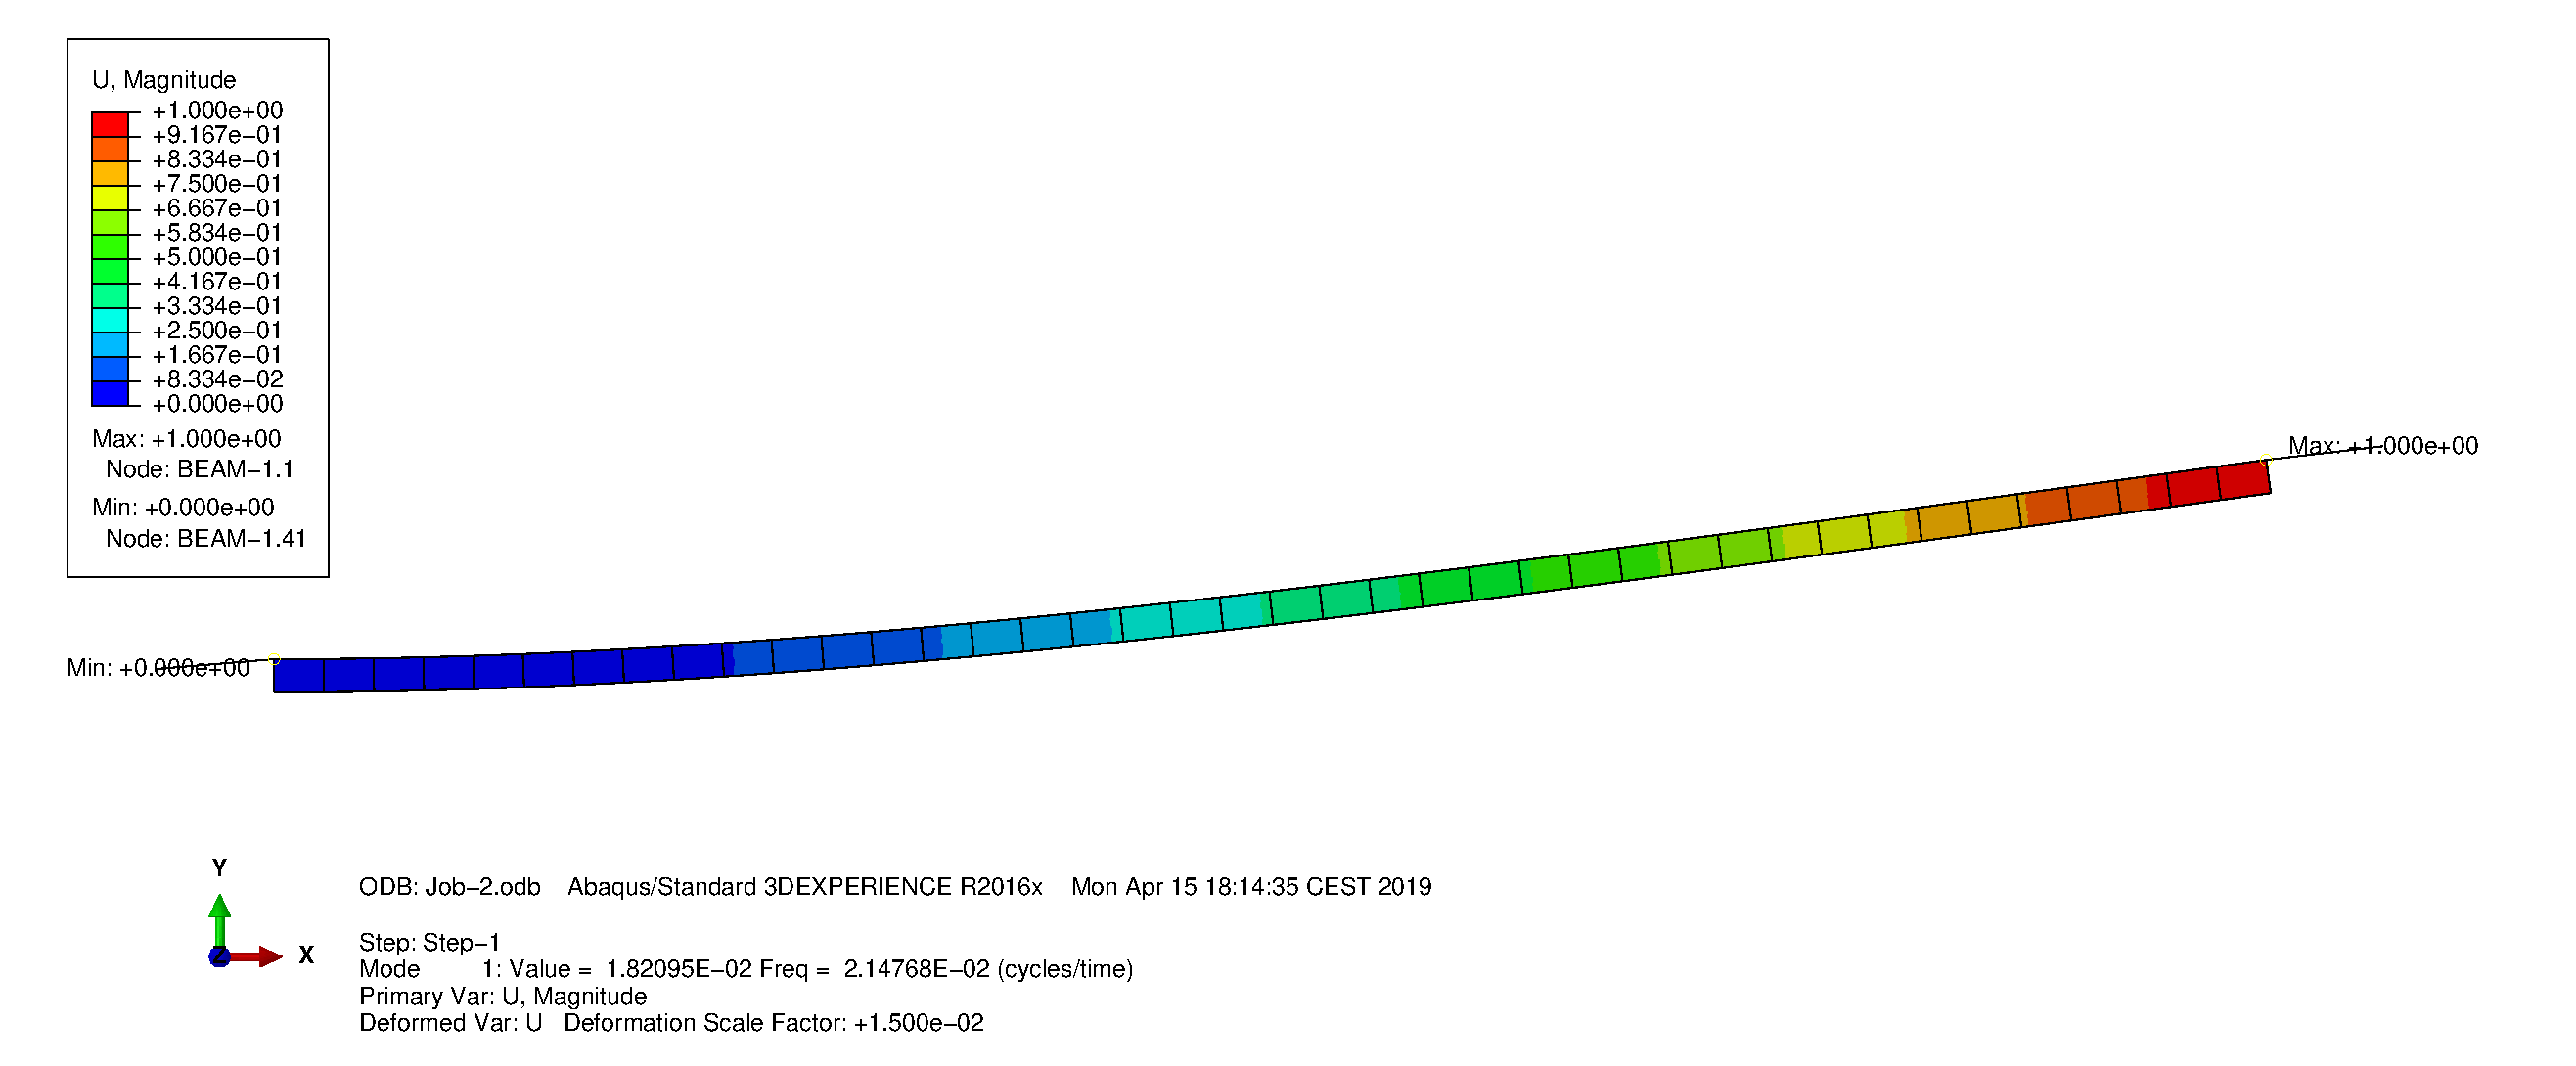
\includegraphics[width=0.95\linewidth]{pics/Beam_1_CPS8R}
    \caption{calculated frequency with CPS4R: 21.4 Hz}
   \end{subfigure}
  \caption{Lower mesh count}
  \label{fig:1}
\end{figure}

\begin{figure}[!htb]
  \centering
  \begin{subfigure}{.5\textwidth}
    \centering
    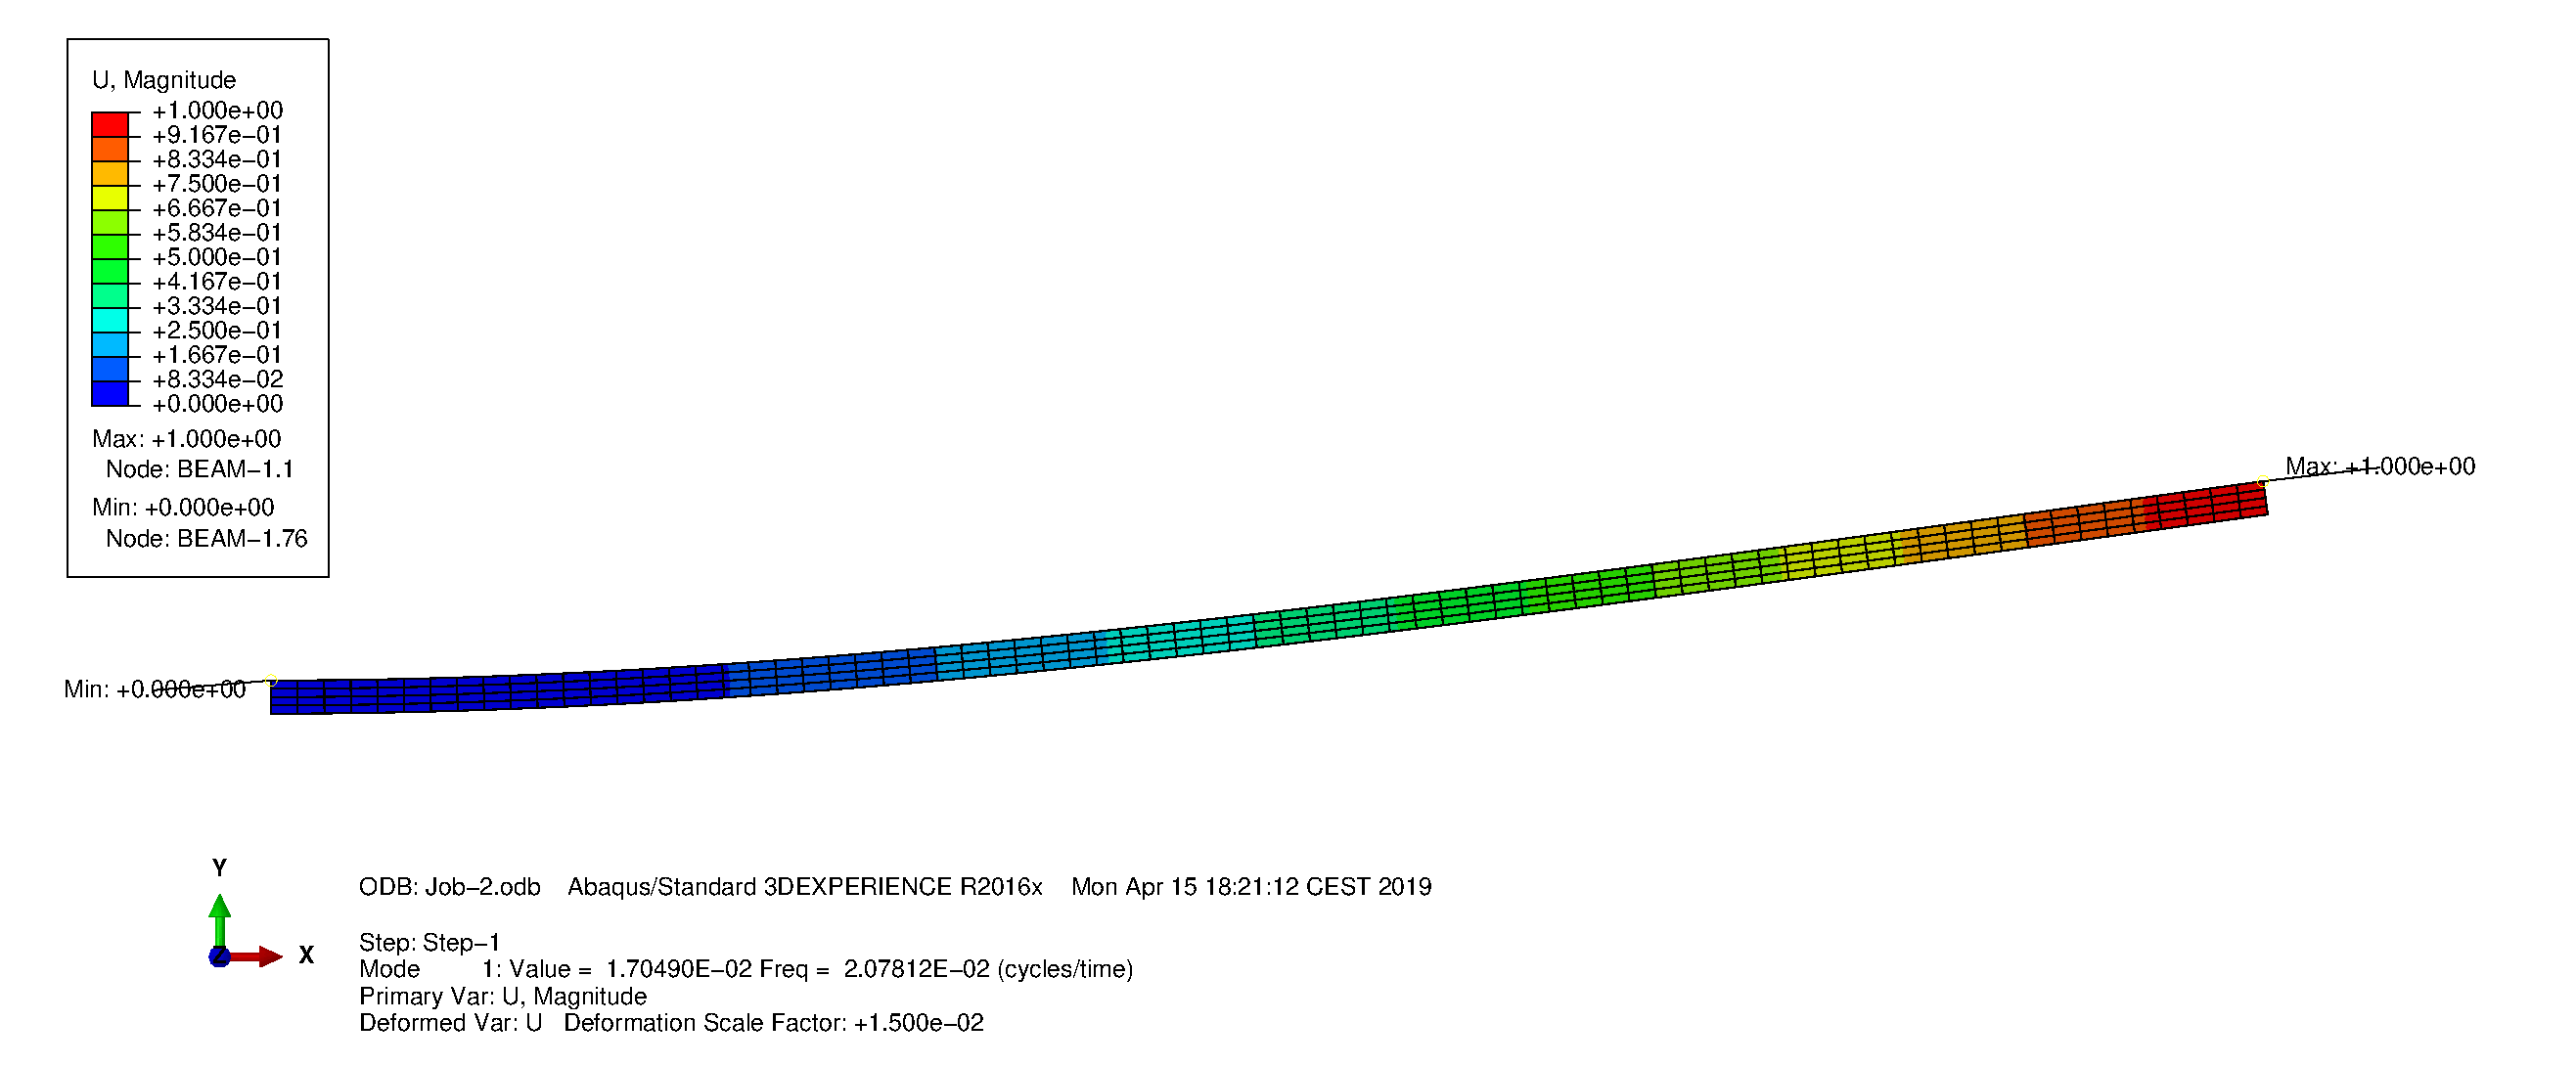
\includegraphics[width=0.95\linewidth]{pics/Beam_1_CPS4R_L}
    \caption{calculated frequency with CPS4R: 20.7 Hz}
  \end{subfigure}%
  \begin{subfigure}{.5\textwidth}
    \centering
    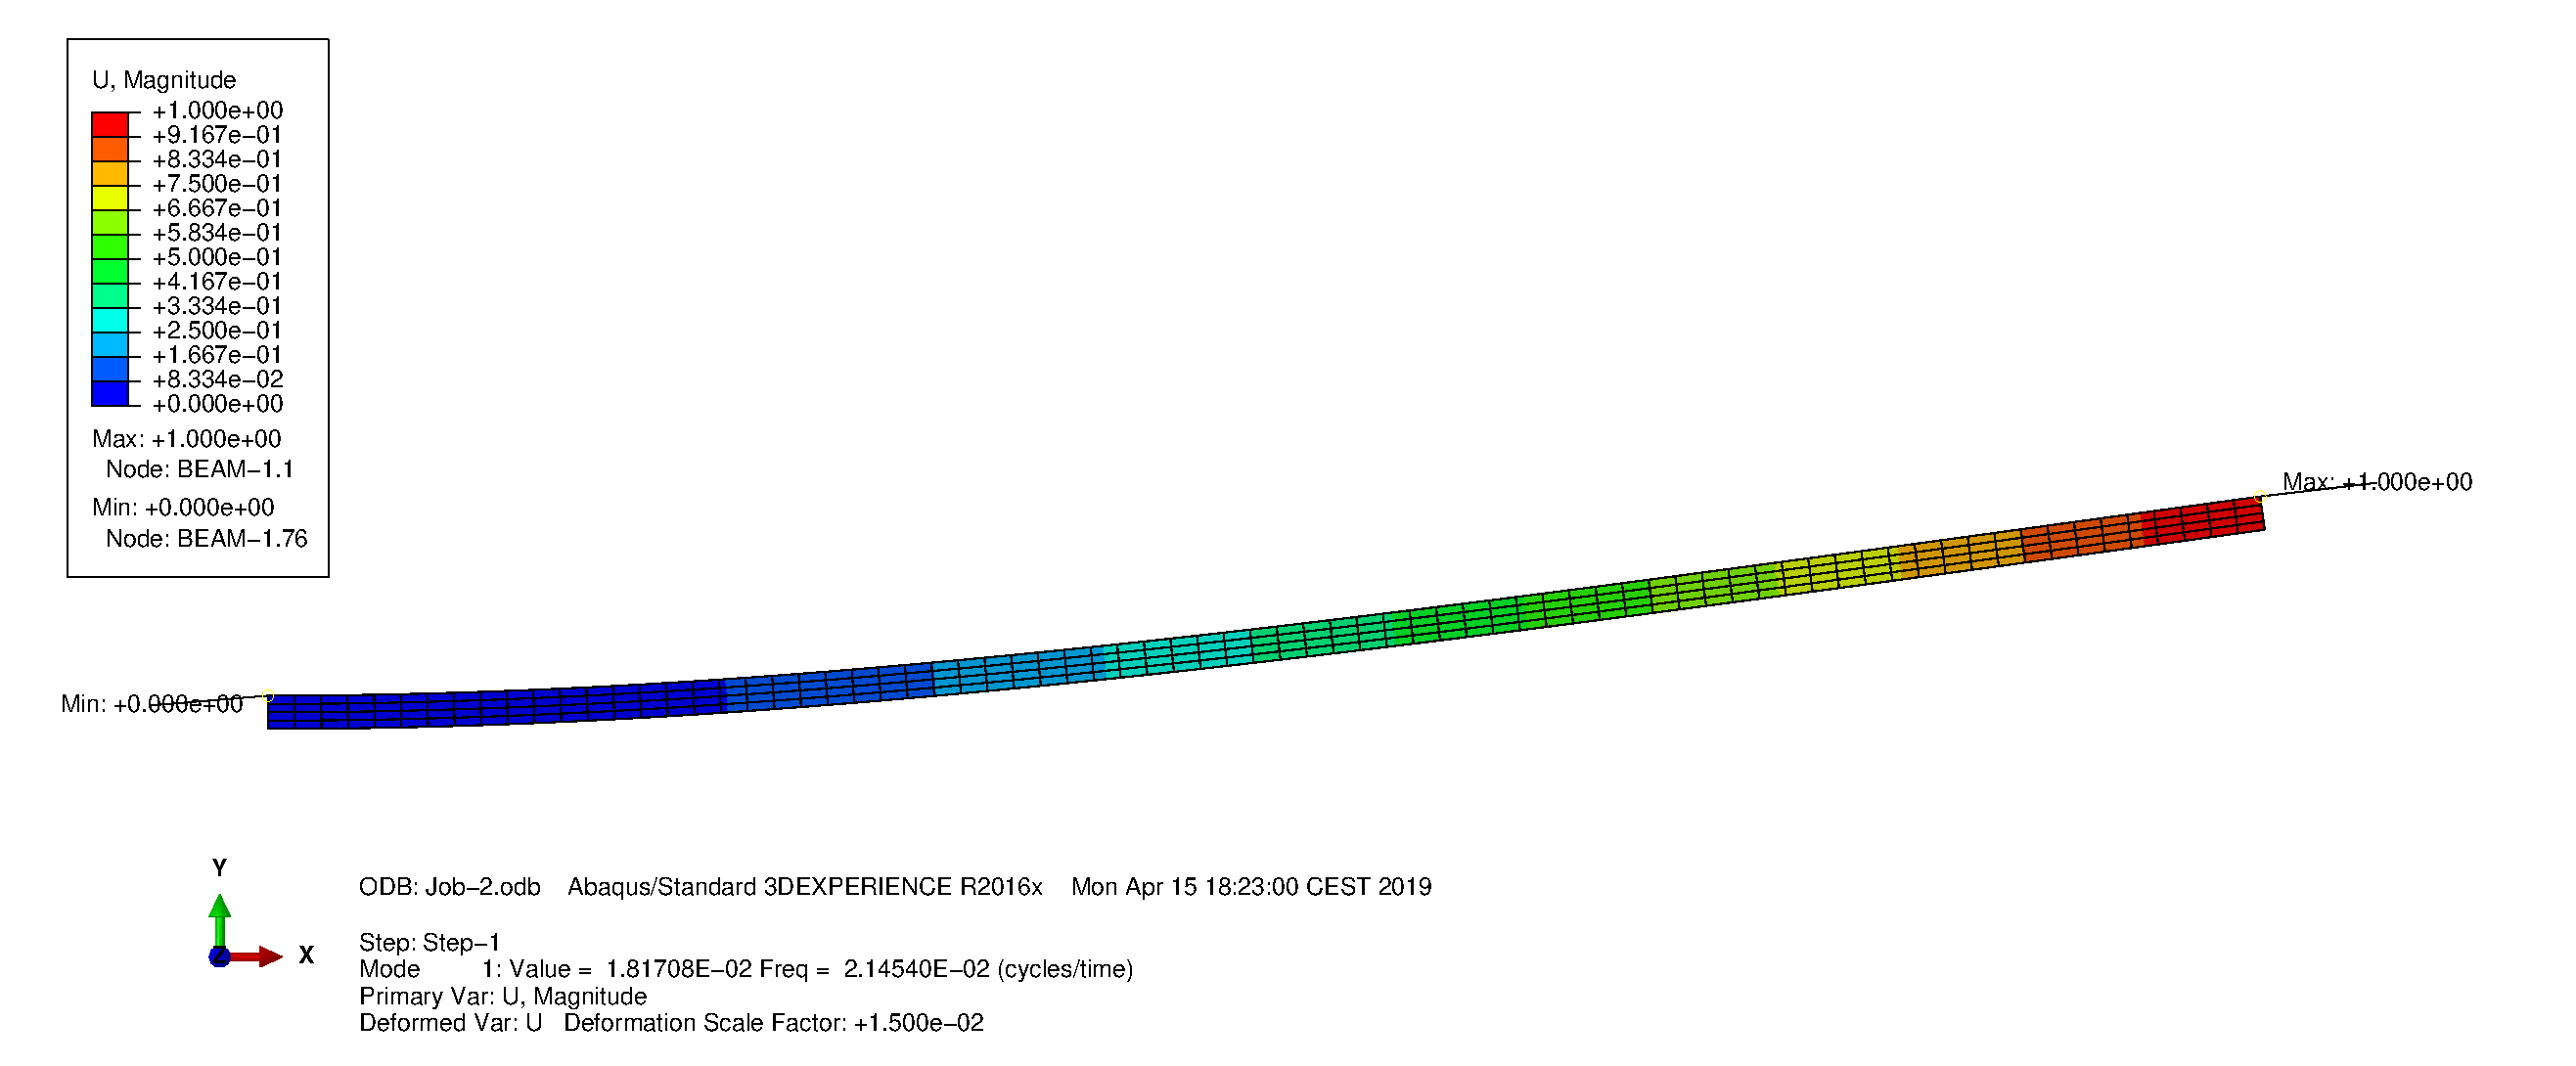
\includegraphics[width=0.95\linewidth]{pics/Beam_1_CPS8R_L}
    \caption{calculated frequency with CPS4R: 21.4 Hz}
   \end{subfigure}
  \caption{Higher mesh count}
  \label{fig:2}
\end{figure}

\noindent Figure \ref{fig:1} shows us the lower mesh count. With (a) using a linar meshing compared to a quadratic one,
we immediately see the better results. This comperation was also discussed in assignment 1. With a higher mesh count,
the differences between the linear and the quadratic method is no so different anymore.
\newpage
\subsection{Generating an impulse}

\begin{figure}[!htb]
  \centering
  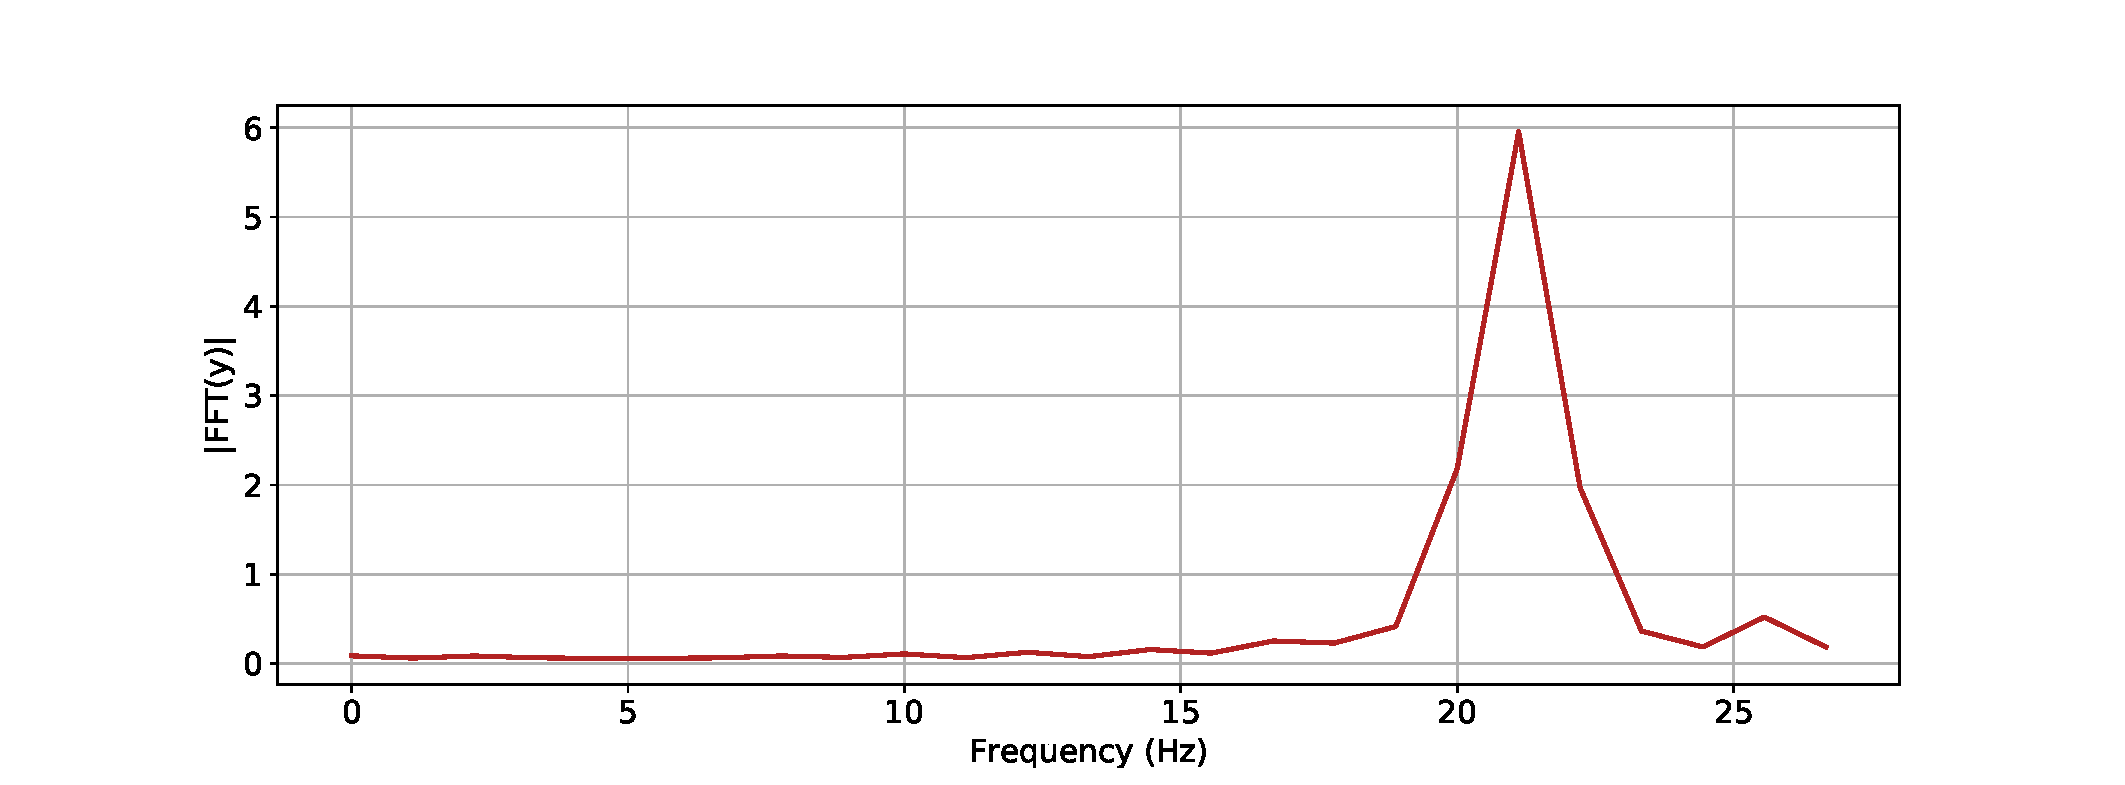
\includegraphics[width=0.95\linewidth]{pics/Report2}
  \caption{Fourier transformation}
\end{figure}

\noindent The impulse on the beam is generated by applying a concentrated force load on the extremity of the beam (the non-encastered end).
This load is being applied for a short time period (1ms). The main advantage is the output, we can not only see one number. With the
Fourier transformation we can also see the distribution of the frequencies and seeing the correct resonannce frequency in the peek of the plot.



\pagebreak
\section{Results and Discussion}

In the submodel with the 1mm fillet, we observe an evenly distributed stress pattern. Also,
the maximum value for stress has decreased by about 50 MPa. From a mechanical point of view, 
the round corner offers a smoother distribution of internal stresses because the lines of 
forces in a material are not interrupted. However, the maximum stress is still the yield 
stress of our material, we still expect it to deform.

\pagebreak
\begin{thebibliography}{9}

  

  \bibitem{latexcompanion} 
  Michel Goossens, Frank Mittelbach, and Alexander Samarin. 
  \textit{The \LaTeX\ Companion}. 
  Addison-Wesley, Reading, Massachusetts, 1993.
   
  \bibitem{einstein} 
  Albert Einstein. 
  \textit{Zur Elektrodynamik bewegter K{\"o}rper}. (German) 
  [\textit{On the electrodynamics of moving bodies}]. 
  Annalen der Physik, 322(10):891–921, 1905.
   
  \bibitem{knuthwebsite} 
  Knuth: Computers and Typesetting,
  \\\texttt{http://www-cs-faculty.stanford.edu/\~{}uno/abcde.html}
\end{thebibliography}


\end{document}